%%
%% cap2.tex
%%
%% Made by Carlos Calcaneo Roldan
%% Login   <calcaneo@jogrant>
%%
%% Started on  Mon Jul 22 15:02:51 2019 Carlos Calcaneo Roldan
%% Last update Time-stamp: <2021-ene-06.miércoles 12:29:37 (Oscar)>
%%

\chapter{Simulaciones Cosmológicas}
\label{chap:2 Sim}
\setcounter{equation}{0}
%%%%%%%%EL Texto Comienza abajo de aquí!

\noindent Las simulaciones cosmológicas son una herramienta esencial para el estudio del Universo. Son el único experimento con el que contamos para reproducir su evolución. Las simulaciones numéricas nos permiten un estudio detallado de formación de estructura no lineal y nos permite hacer conexiones entre un Universo simple, es decir, aquel con alto corrimiento al rojo y con uno complejo, como el que se observa en la actualidad.

El trabajo que se realiza va desde el estudio del agrupamiento gravitacional no lineal de materia oscura, formación de grupos de galaxias, interacción de galaxias aisladas y la evolución de gas intergaláctico. Su desarrollo ha permitido un inmenso avance en estas áreas, el cual no era posible antes dado a las limitaciones que existían en el computó \cite{2001NewA....6...79S}.


Con la rápida evolución en el rendimiento de las computadoras y algoritmos numéricos, han nacido múltiples códigos que simulan la formación de estructura del Universo. Entendemos por estructura a la red complicada de cúmulos de galaxias, galaxias y hasta cúmulos de estrellas los cuales, dependiendo de la escala que estudiamos, sera la estructura o sub-estructura (asi, por ejemplo las galaxias son parte de la subestructura de los cúmulos de galaxias).

Muchos de estos códigos se han hecho públicos y libres, lo que ha permitido que el estudio sea mas sencillo para nuevos investigadores o grupos de investigación \cite{2021MNRAS.506.2871S}. El futuro de las simulaciones numéricas esta en hacer mejoras en la precisión y en la fidelidad en la Física de las técnicas de modelado.

\newpage

\section{Grandes Simulaciones}

Gracias al desarrollo de códigos y el avance en el hardware de las maquinas modernas, han surgido grandes colaboraciones con la intención de realizar simulaciones cada vez mas grandes. Algunas de ellas son:

%==================================================================================================
%==================================================================================================
%==================================================================================================
\subsubsection{Millennium Simulation}

La Millennium Simulation fue una de las mas grandes simulaciones de N-Cuerpos realizada en el 2005. Esta contenía mas de 10 billones de partículas en una caja de 2 billones de años luz por lado. La simulación se realizó por la Virgo Consortium usando 512 procesadores localizados en el Instituto Max Planck para Astrofísica en Garching, Alemania. Tomo 28 días (~600 horas), consumiendo alrededor de 343,000 horas de tiempo de cpu \cite{2005Natur.435..629S}.

Esta fue la primera simulación parte de una serie de simulaciones relacionadas a volúmenes cosmológicos. En 2008 se realizó una segunda simulación con las misma cosmología, misma estructura de salida y misma cantidad de partículas, pero con una caja 5 veces mas pequeña, lo que aumento la densidad de partículas y por tanto permitió tener una resolución de masa 125 veces mejor.

\begin{figure}[H]
    \centering
    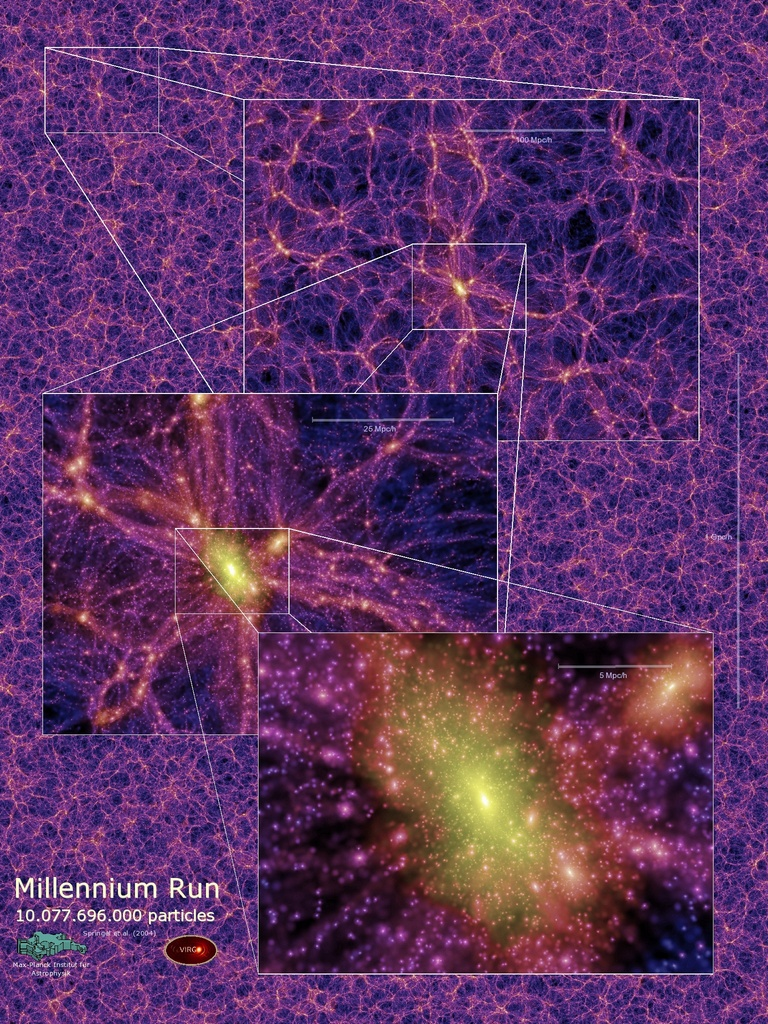
\includegraphics[width = 0.35\linewidth]{Millenium-Sim.jpg}
    \caption[Millennium Simulation Cosmic Web]{Se muestra el mapa de densidad de un corte de $15 Mpc/h$ en redshift $z=0$ de la \textit{Millennium Simulation}. Imagen obtenida de MPA}
    \label{fig:Millennium_Sim}
\end{figure}


%==================================================================================================
%==================================================================================================
%==================================================================================================
\subsubsection{Eagle Simulation}
El proyecto EAGLE (Evolution and Assembly of GaLaxies and their Environments)  es una colaboración de The Virgo Consortium, la cual es una simulación hidrodinámica de gran escala de un Universo de $\Lambda$CDM, el cual tenia como objetivo entender como las galaxias se forman y evolucionan. La mas grande de las simulaciones se realizo con  6.8 billones de partículas, en un volumen de 100 Mpc por lado, conteniendo al menos 10,000 galaxias del tamaño de la vía láctea, la cual tardo mas de un mes y medio de tiempo de computo y una de la mas grandes super-computadoras con 4000 núcleos de procesamiento usando una versión modificada del código de simulación GADGET-2 \cite{2015MNRAS.450.1937C, 2015MNRAS.446..521S}.

La simulación empieza en un Universo todavía muy uniforme (sin formación de estrellas o galaxias) usando parámetros motivados por las observaciones del satélite Plank \cite{ 2013ApJS..208...20B, 2020A&A...641A...1P}. Algunos de los parámetros cruciales de la simulación son la densidad de materia oscura, la cual es responsable de la formación de estructura de materia bariónica, así como la constante cosmológica, responsable de la expansión acelerada del Universo.
       
\begin{figure}[H]
    \centering
    \includegraphics[width = 0.45\linewidth]{Eagle-Sim.png}
    \caption[Eagle Simulation Cosmic Web]{Se muestra el mapa de densidad de la Eagle Simulation. Obtenida de \textit{The Eagle Project} }
    \label{fig:Eagle_Sim}
\end{figure}

%==================================================================================================
%==================================================================================================
%==================================================================================================
Es eviente de las figuras \ref{fig:Millennium_Sim} \ref{fig:Eagle_Sim}, Como en las simulaciones cosmológicas las partículas se aglomeran para formar grupos cada vez mas grandes. Al inicio (en un alto corriemito al rojo) las simulación tiene una denisdad muy uniforme,conforme avanza el tiempo vemos quer se generan agrupaciones esfericas entrelazdas con una red de denisdad de particulas. A toda esta complejidad en la distribución de la densidad de partículas en la simulación le llamamos también estructura. Al fijarnos con detalle en una coleción esferica grande con respecto al volumen de las simulación notamos que tambien se forman pequeños grupos, los seran ahora la sub-estructura.
%==================================================================================================
%==================================================================================================
%==================================================================================================
\section{La interacción dominante en las simulaciones}

Para estudiar el comportamiento de un sistema de partículas, tenemos que simplificarlo la mas posible. Empezamos identificando la fuerza responsable del movimiento de las partículas, en este caso es la gravedad y en específico nos quedamos con la gravedad descrita por Newton \eqref{eq:Gravedad-Newton}. Por tanto, solo requerimos conocer las masas y las posiciones de las partículas.

\begin{equation}
    F = G \frac{m_1 m_2}{r^2}
    \label{eq:Gravedad-Newton}
\end{equation}

Pero como estamos tratando con sistema de $N$ partículas tenemos que considerar la contribución de fuerzas debida al resto de las partículas. Por el teorema de superposición podemos decir que
\begin{equation}
    F_{1} = F_{1,2} +F_{1,3} + \dots + F_{1,N} = \sum_{i=2}^{N} F_{1,i} 
    \label{eq:superposicion}
\end{equation}

Pero también podemos resolver el problema si trabajamos con el potencial
\begin{equation}
    \nabla \phi(\mathbf{r}) = \mathbf{F}
    \label{eq:potencial-gravitacional}
\end{equation}

%==================================================================================================
%==================================================================================================
%==================================================================================================
\section{Una razón práctica para las simulaciones}

Si consideramos las dimensiones de nuestra galaxia, podemos calcular el camino medio libre de una estrella antes de que colisione con otra estrella. En un sistema de partículas que se mueven en orbitas rectas, el camino medio libre es $\lambda = 1/(n\sigma)$ donde $n$ es la densidad numérica de partículas y $\sigma$ es la sección transversal de cada estrella. Asumiendo que todas las estrellas son como nuestro sol ($\sigma = \pi(2R_\odot)^2 $ donde $R_\odot = 6.96\times 10^{10}$ cm) y teniendo que en la galaxia hay aproximadamente $10^{11}$ estrellas distribuidas uniformemente sobre un disco de radio de $10 kpc$ y grosor de $1 kpc$, tenemos una densidad de numero de estrellas en el disco de $n=0.3pc^{-3}$. Por lo tanto el camino medio libre es de $\lambda = 1.5 \times 10^{33} cm = 5\times 10^{14}pc$. Ahora el tiempo entre colisiones es aproximadamente $\lambda / v$, donde $v$ es la velocidad aleatoria de una estrella en un lugar dado. Para $v=40km s^{-1}$ el intervalo entre colisiones es aproximadamente de $10^{19}$ años, $10^9$ veces mas antiguo que la edad de la galaxia \cite{Binney1988-rs}. Es evidente que las colisiones entre estrellas son lo suficientemente raras que no tienen importancia en la dinámica de las galaxias, por lo que para cualquier propósito, la dinámica de las estrellas en la galaxia se pueden aproximar a la de un conjunto de puntos masivos que no colisionan entre si, es decir un gas sin colisiones.

Como vemos que las colisiones entre estrellas de una galaxia son raras, podemos decir que a la escala del Universo sucede lo mismo. Por lo tanto, si queremos simular nuestro Universo, idealmente se debe resolver la ecuación de Boltzmann sin colisiones (CBE)

\begin{equation}
    \frac{d f}{d t} \equiv \frac{\partial f}{\partial t} + \mathbf{v}\frac{\partial f}{\partial \mathbf{x}} + \frac{\partial \Phi}{\partial \mathbf{r}} \frac{\partial f}{\partial \mathbf{v}}
    \label{eq:CBE}
\end{equation}

\noindent donde el potencial auto-consistente $\Phi$ es la solución a la ecuación de Poisson

\begin{equation}
    \nabla^2\Phi(\mathbf{r},t) = 4\pi G \int f(\mathbf{r},\mathbf{v},t)d\mathbf{v}
    \label{eq:PoissonSol}
\end{equation}

\noindent y $f(\mathbf{r},\mathbf{v},t)$ es la densidad de partículas en el espacio fase.

% En la práctica, no resolvemos CBE, sino que representamos el Universo como un sistema de N partículas, por lo tanto, se transforma en un problema de N-Cuerpos donde se siguen las ecuaciones de movimiento de Newton. Notemos que ahora es necesario introducir un radio de suavizado para pequeñas distancias con el objetivo de evitar que en el caso de una colisión de dos cuerpos, las partículas no salgan disparadas y para mantener el sistema sin colisiones. Según el número de partículas con el que se va a trabajar, va tener un efecto sobre como escoger el radio de suavizado.


% Pero lo que se realiza para simular nuestro Universo no es resolver CBE, si no que optamos por trabajar con un sistema de N-Cuerpos y ver 

% Es muy complicado resolver este sistema de ecuaciones. La solución a la que se a llegado es construir códigos para simulaciones de N-Cuerpos. Existen grandes cantidades de códigos para simulaciones de N-Cuerpos, pero se diferencian en como realizan los cálculos para el movimiento gravitacional. Además de que siempre están buscando la forma de hacer los simuladores mas rápidos y eficientes.

Seguir esta ruta presenta algunos retos tanto computacionales como físicos ya que debemos conocer bien la densidad en el espacio fase. Esta cantidad es prácticamente imposible de conocer para el Universo temprano, aunque se hacen algunos intentos por extrapolar posibles formas a partir de estructuras que vemos en el cielo actualmente (ver por ejemplo, [\cite[Binney]{Binney1988-rs} ], capítulo 7). 

La solución que se ha preferido es aproximar la dinámica mediante códigos de N-cuerpos, en los cuales se supone una interacción entre partículas dada por la interacción gravitacional clásica por pares de partículas en las cuales se agrega un radio de suavizado para evitar dividir por cero cuando se acercan mucho los cuerpos. 

Existen grandes cantidades de códigos para simulaciones de N-Cuerpos, pero se diferencian en como realizan los cálculos para el movimiento gravitacional. Además de que siempre están buscando la forma de hacer los simuladores mas rápidos y eficientes.
%==================================================================================================
%==================================================================================================
%==================================================================================================

\section{GADGET-4}
% Las simulaciones numéricas permiten el estudio detallado de formación de estructura y conecta a un Universo simple con alto corrimiento al rojo con uno con estructura compleja como la que se observa en la actualidad. 

Los código GADGET han sido de los mas utilizados en el estudió de formación de estructura y estudio de la materia oscura en las ultimas dos décadas. Han existido varias iteraciones de los códigos GADGET, siendo GADGET-4 la mas reciente y una renovación completa del simulador. 

La motivación detrás de la nueva versión de GADGET-4 fue construir un simulador con el cual se pudieran tener simulaciones mas grandes y con mayor precisión. Esto implica tener cálculos con gran poder estadístico y mayor resolución y para lograr esto, GADGET-4 hace uso de métodos de paralelización avanzados. Pero debido a la necesidad de tener simulaciones cada vez mas grandes, se ha buscado mejorar escalabilidad del código GADGET-4 \cite{2021MNRAS.506.2871S}.

Para grandes simulaciones, se procura tener un buen rendimiento en condiciones de alto rango dinámico en escalas de tiempo. También busca mejorar la precisión en los cálculos de fuerza gravitacional e hidrodinámica. Finalmente se buscó modernizar el código, quitando partes obsoletas y mejorando la legibilidad y la modularidad del código con el objetivo de que los usuarios puedan desarrollar con facilidad extensiones para el mismo. 

 
Una de las características que separa a GADGET-4 de otros simuladores, es que es un código flexible multi-propósito que no restringe el tipo de simulaciones, sino que da prioridad a la flexibilidad  sobre la optimización para casos específicos. Para esto se implementaron un buen numero de nuevos métodos numéricos. También se introdujeron nuevas funcionalidades al código en la forma de la introducción de código para la búsqueda de grupos y sub-estructura (\textit{Friends of Friends} (FOF), SUBFIND) asi como un \textit{Merger Tree} que corre junto a la simulación. Se incluyo una nueva variación de un buscador de sub-estructura, SUBFIND-HBT, que usa la información de sub-halos del pasado en consideración, lo que permite una forma robusta y eficiente de seguir la sub-estructura en el tiempo incluso después de unirse a otro halo. GADGET-4 también es capaz de generar sus condiciones iniciales ya sea usando la aproximación de Zeldovich o con la teoría de la perturbación lagrangiana de segundo orden (2PLT)\cite{2021MNRAS.506.2871S}.


\subsubsection{Cálculos de Gravedad de GADGET-4}

Tenemos un potencial $\Phi (\mathbf{x})$ producido por $N$ partículas con masas $m_j$ en coordenadas $x_j$ en el dominio con dimensiones $L_x \times L_y \times L_z$ que se replica periódicamente en las tres direcciones esta dado por:

\begin{equation}
    \Phi (\mathbf{x}) = - \sum_{j=1}^{N} \sum_{\mathbf{n}=-\infty}^{\infty}  \frac{ m_j }{ |\mathbf{x}_j - \mathbf{x} + \mathbf{q}_n| + |\epsilon ( \mathbf{x}_j - \mathbf{x} + \mathbf{q}_n)| }   - m_j\varphi_{\mathbf{n}}(\mathbf{x})
    \label{eq:Grav_Pot_1}
\end{equation}

\noindent donde $\mathbf{q_n}$ denota vectores de desplazamiento periódico dados por $\mathbf{q}_n$=($n_x$$L_x$,$ n_y$$L_y$,$n_z$$L_z$) y $\mathbf{n} = (n_x, n_y, n_z)$ son tripletes enteros y la suma sobre $\mathbf{n}$ se extiende sobre todo los tripletes. Se omitió la constante gravitacional $G$ por simplicidad. La contribución del potencial $\varphi_{\mathbf{n}}(\mathbf{x})$ es el de un cubo homogéneo de unidad de masa y extensión $L_x \times L_y \times L_z$ con un desplazamiento $\mathbf{q_n}$. Este termino se agrega para que la suma converja sobre un sistema periódico, de manera que efectivamente se establece neutralidad de carga gravitacional.

La función $\epsilon(r)$ describe a la ley de suavizado gravitacional. Debemos asumir que el suavizado tiene un rango finito, donde $\epsilon(r)=0$ para $r\geq r_0$ y donde $r_0$ es mas pequeño que la mitad de la dimensión mas pequeña de la caja. En GADGET-4 se ha adoptado un potencial donde el potencial de una partícula puntual se remplaza por un potencial con una distribución de masa suave con bordes en $h=2.8\epsilon_0$, donde $\epsilon_0$ es el radio de suavizado. La ley de suavizado esta dada por:

\begin{equation}
    \epsilon(r;\epsilon_0) = - \frac{2.8\epsilon_0}{W_2(r/2.8\epsilon_0)} -r
    \label{eq:Ley-Suavizado}
\end{equation}

Ahora definamos $\mathbf{q}^*_j(x)$ como el desplazamiento periódico que minimiza la distancia de $\mathbf{x}_j+\mathbf{q}_n$ a $x$ (es decir selecciona la ubicación de la partícula $j$ imagen periódica mas cercana a la posición $\mathbf{x}$), podemos escribir el potencial como:
% Esencialmente para resolver el sistema de N-cuerpos, el potencial gravitacional que se usa para calcular el movimiento de las N partículas es el siguiente:

\begin{align}
    \Phi (\textbf{x}) = &- \sum_{j=1}^{N} \frac{m_j}{|\textbf{x}_j-\textbf{x}+\textbf{q}^*_j| + |\epsilon(\textbf{x}_j-\textbf{x}+\textbf{q}^*_j)|} \nonumber \\
    &+ \sum_{j=1}^{N} m_j \psi (\textbf{x}_j-\textbf{x}+\textbf{q}^*_j) \label{eq:Pot}
\end{align}

\noindent donde la primera parte es el potencial gravitacional de newton con una corrección para considerar el radio de suavizado y el segundo termino en potencial se introduce como una corrección para el suavizado de imágenes distantes. Este es el potencial que GADGET-4 usa como base para los cálculos de gravedad, pero como GADGET-4 es un simulador diseñado para abarcar una amplia gama de necesidades, sus desarrolladores implementaron diversos algoritmos para la forma en la que se realizaron los cálculos.


\subsubsection{Buscador de grupos y sub-halos}

Las simulaciones cosmológicas son una herramienta util para simular el movimiento de cuerpos en nuestro Universo, pero ocupamos mas herramientas para poder describir las propiedades del Universo. En GADGET-4 se han implementado una diversa cantidad de herramientas con las que podemos estudiar nuestras simulaciones y muchas de estas corren junto a la simulación, lo que permite tener mejores resultados. Algunas de las herramientas que tiene GADGET-4 son buscador de grupos y sub-halos, construcción de arboles de fusión, conos de luz, estimación del espectro de potencia y generación de condiciones iniciales. 

La herramienta de nuestro interés fue el buscador de grupos y sub-halos. GADGET-4 tiene tres implementaciones distintas. Se implementó un \textit{Friends of Friends} (FOF), un algoritmo SUBFIND para buscar sub-estructura ligada gravitacionalmente y nueva variante SUBFIND-HBT el cual usa información pasada de miembros del grupos para ver la evolución de los grupos y sub-halos.

\subsubsection{ Friends of Friends (\textbf{FOF}) }
El algoritmo de FOF organiza los halos en una lista de enlaces. Este empieza poniendo todas las partículas en su propio grupo, luego el se busca todos los pares de partículas con una distancia menor a longitud de enlace $l$. El valor mas común de $l$ es $0.2$ veces la distancia media entre partícula. De esta manera los halos están ligados por contornos de densidad que aproximan sobre-densidades. Cada par que se encuentra con una distancia suficiente pequeña, provoca que los grupos a los que pertenecen se unan. La implementación de GADGET-4 se ha reportado tener mayores velocidades comparados con otras implementaciones en la literatura \cite{2021MNRAS.506.2871S}.

\subsubsection{SUBFIND}
En la búsqueda de estructuras de materia oscura, el buscador FOF se puede combinar con el algoritmo SUBFIND. La idea es checar si los halos encontrados son estructuras ligadas gravitacionalmente. Primero se busca el campo de densidad, donde se busca picos de densidad aislados. De ahi se buscan los puntos sillas que conectan dos picos de densidad. El pico pequeño se registra como un candidato de sub-estructura, el cual se somete a un procedimiento con el cual se verifica que se encuentra ligado gravitacionalmente. 

En la implementación que se realizó en GADGET-4, para la selección de cuales picos son sub-estructura y cuales solo están en el fondo (no forman parte de la sub-estructura), se puede tomar en cuenta la historia de las partículas sobre a cuales halos formo parte en el pasado. Esto lo puede hacer mientras se evoluciona el sistema de la simulación tomando en cuenta a que halos han pertenecido y la suma acumulada del tamaño del halo, mientras que en el si se realiza al terminar la simulación esta información se recolecta de los snapshots en orden temporal. El pico con la mayor suma se identifica como un pico del fondo (no es necesariamente el pico con la mayor cantidad de partículas).

\subsubsection{SUBFIND-HBT}
Hemos visto dos herramientas que nos permiten identificar estructuras, cada una con una aproximación diferente para determinar la pertenencia de las partículas a estructura. Ahora veremos la última implementación de buscador de estructura que tiene GADGET-4. SUBFIND identifica estructura ligada gravitacionalmente en el espacio coordenado en un solo corte temporal. Este método tiende a ser demandante computacionalmente y tiende a tener problemas identificando toda la materia que contiene la sub-estructura, especialmente cerca del pericentro del subhalo que orbita un halo mas grande. 

Este método tiende a ser muy rápido ya que suele omitir el paso donde verifican si las partículas se encuentran ligadas gravitacionalmente, lo que hace que las estructuras identificadas tengan una naturaleza física no definida seguramente. Una alternativa es depender de información pasada para la identificación de halos. Si tenemos un conjunto de partículas que se encuentran ligadas gravitacionalmente y se clasifica como una sub-estructura de un sistema mas grande, se puede checar continuamente si las partículas siguen ligadas. Esto asume que las estructuras solo pueden perder partículas y que no crecen en masa en una manera apreciable cuando se encuentra en órbita de un sistema mas grande. Este algoritmo se le conoce como \textit{Hierarchically Bound Tracing}(HBT).

GADGET-4 implemento una variante de HBT+. En la practica, este algoritmo puede reemplazar a SUBFIND teniendo la misma estructura de salida, a este enfoque SUBFIND-HBT. Funciona solamente con los snapshots en secuencia procesados en orden temporal. El método primeramente encuentra nuevos grupos FOF. Después se identifican candidatos para sub-estructura en cada grupo FOF basados en su pasadas afiliaciones de sub-estructuras. Los candidatos mas grandes encontrados se descartan por el momento, debido a que el procedimiento lo identifica como el halo del fondo del grupo, el cual puede crecer en masa. El resto de los candidatos se someten a un proceso para identificar si las partículas siguen ligas a la sub-estructura usando sus coordenadas en el espacio fase. Este método es significativamente mas simple y barato computacionalmente ya que no se necesita calcular el campo de densidad y por tanto no hay necesidad de procesar el calculo de los puntos sillas. La gran ventaja es que capaz de recuperar la masa total de todas las sub-estructuras, incluso de las que están cerca del pericentro en su orbita \cite{2021MNRAS.506.2871S}.